\documentclass[sigconf,nonacm]{acmart}

% current version: v2

% -----------------------------------------------------------------------------
% POSID / InciText arXiv revision
% Drafting rule for this revision:
%   - rewrite one section at a time;
%   - do not invent experimental values;
%   - when a planned table/figure is not yet supported by a frozen run,
%     keep the artifact in the manuscript with blank cells / placeholder content.
% -----------------------------------------------------------------------------

\usepackage{booktabs}
\usepackage{multirow}
\usepackage{amsmath}
\usepackage[ruled,vlined,linesnumbered,noend]{algorithm2e}
\usepackage{subcaption}
\usepackage{enumitem}
\usepackage{xurl}
\usepackage{balance}
\usepackage{tikz}
\usetikzlibrary{arrows.meta,positioning,fit}

\newcommand{\posid}{\textsc{POSID}}
\newcommand{\incitext}{\textsc{InciText}}
\newcommand{\blankresult}{\phantom{0.00}}

\title{A Modular Unsupervised Framework for Attribute Recognition from Unstructured Text}

\author{KMA Solaiman}
% TODO(author): Confirm the affiliation to display on the next arXiv version.
\affiliation{%
  \institution{Purdue University}
  \city{West Lafayette}
  \state{Indiana}
  \country{USA}
}
\email{ksolaima@umbc.edu}

\begin{document}

% Keep the abstract stable while the body is rewritten section-by-section.
% Rewrite it only after the method, evaluation protocol, and final reported
% results are frozen.
\begin{abstract}
We propose \posid, a modular and lightweight framework for extracting structured
attribute--value descriptions from unstructured text without task-specific
supervised training. The framework first identifies candidate text spans using
lexical, semantic, or zero-shot candidate selectors and then applies a
structured extraction procedure to recover attributes and their values. We use
human attribute recognition in heterogeneous public-safety text as the primary
case study and evaluate the approach on the \incitext{} dataset. The present
study focuses on extracting explicitly stated person attributes, including
gender, race, height, and clothing descriptions, without training or fine-tuning
on labeled \incitext{} examples.
\end{abstract}

\maketitle

% =============================================================================
% SECTION 1 -- REWRITTEN
% =============================================================================
\section{Introduction}
\label{sec:introduction}

Structured descriptions of people are frequently embedded in free-form text.
An incident report, dispatch record, press release, missing-person notice, or
other public-safety narrative may describe a person through attributes such as
gender, race, height, build, clothing items, and clothing descriptors. These
facts are useful only after they have been associated with the described person
and converted from prose into a consistent structured representation. We study
this problem as \emph{attribute recognition from text}: given a document, first
locate the text that contains relevant descriptions and then recover the
corresponding attribute--value pairs.

The difficulty is not only that the input is unstructured. The source documents
can differ substantially in genre, layout, sentence structure, abbreviations,
and the location and density of attribute evidence. Some descriptions are
compact (e.g., a demographic phrase followed by clothing); others distribute
attributes across neighboring sentences or embed them in longer narratives.
Fixed-vocabulary attributes such as gender can often be recognized with
constrained lexical patterns, while variable-valued attributes such as clothing
require recovering an open-ended set of item names and their modifiers. A
single extraction strategy therefore has to cope with both variation in
\emph{where} useful evidence appears and variation in \emph{how} an attribute is
expressed.


A conventional approach could formulate the task as supervised sequence
labeling, relation extraction, or question answering, provided enough labeled
examples are available. Our setting instead asks how much structured
information can be recovered \emph{without task-specific supervised training}.
Throughout this paper, we use \emph{unsupervised} in this target-task sense:
\posid{} is not trained or fine-tuned on labeled \incitext{} examples. Individual
pretrained components may themselves have been trained on external corpora or
external tasks. In particular, one candidate selector uses a pretrained
natural-language-inference model in a zero-shot configuration. This distinction
is important: the framework avoids supervision for the attribute-recognition
task while still permitting reusable pretrained representations.

We propose \posid{} as a modular two-stage framework. The first stage performs
\emph{candidate retrieval}: it identifies sentences or sentence fragments that
are likely to contain relevant person descriptions. Candidate selectors may be
lexical or semantic, including regular-expression matching, Word2Vec
similarity~\cite{mikolov2013efficient}, WordNet similarity~\cite{wordnet98}, and
zero-shot natural-language inference. The second stage performs
\emph{structured extraction}: it uses attribute-specific lexical constraints,
local context, part-of-speech information, and lightweight semantic checks to
recover attribute values and associate them with person mentions. Separating
candidate retrieval from structured extraction makes the retrieval mechanism a
replaceable front end rather than embedding one retrieval assumption throughout
the extraction algorithm.

The separation is particularly useful for clothing descriptions. A precise
lexical cue can strongly localize the relevant span, whereas a semantic
candidate selector can recover descriptions that do not use the expected cue.
After localization, however, not every noun or modifier in the candidate is
necessarily part of a clothing description. This creates a second source of
uncertainty inside the candidate itself: the extractor must decide when the
local syntactic evidence remains sufficient to continue parsing and when it
should stop. We therefore treat candidate relevance and extraction reliability
as separate decisions rather than assuming that a semantically relevant
sentence can be parsed exhaustively.

Human attribute recognition is used here as a concrete case study for this
architecture. We evaluate \posid{} on \incitext{}, which contains heterogeneous
public-safety text and person-level annotations. The current 28-document
historical subset is used as a small proof-of-concept evaluation spanning
multiple source styles; the dataset and evaluation units are defined explicitly
in Section~\ref{sec:dataset}. We do not use this small study to claim general
cross-domain robustness. Instead, it establishes whether the proposed modular
pipeline can recover structured attributes under the textual variation present
in the available corpus.

The contributions of this paper are:
\begin{enumerate}[leftmargin=*,itemsep=2pt,topsep=3pt]
    \item We formulate person-attribute extraction from heterogeneous
    public-safety text as two separable stages---candidate localization and
    structured attribute recovery---and present \posid{}, a
    target-task-unsupervised framework in which lexical, distributional, and
    zero-shot semantic selectors feed a common POS-guided extractor for fixed
    attributes and open-vocabulary clothing descriptions.

    \item We conduct a controlled comparison of RE, Word2Vec, WordNet,
    zero-shot NLI, and routed combinations under the same downstream recovery
    layer, allowing candidate-selection behavior to be studied without changing
    the structured extractor.

    \item We identify syntactic termination as a distinct extraction decision
    after candidate localization and empirically compare conservative early
    stopping with permissive continuation. The results expose a
    selector-dependent precision--recall tradeoff and show that locating a
    relevant candidate does not imply that all subsequent candidate text should
    be consumed as attribute evidence.
\end{enumerate}

% =============================================================================
% Remaining sections -- intentionally not rewritten yet.
% These headings define the working paper structure so main.tex compiles while
% we revise one section at a time.
% =============================================================================

\section{The \incitext{} Dataset}
\label{sec:dataset}

\incitext{} is a person-attribute text corpus assembled from public-safety
documents and controlled text generation. The corpus is heterogeneous by
construction: its sources differ in length, layout, writing style, degree of
structure, and the location of person-description evidence. Because the
experiments in this paper use only a small source-derived portion of the
available data, we distinguish throughout this section between the
\emph{consolidated corpus inventory} and the \emph{28-document
proof-of-concept subset} used in the present evaluation.

\subsection{Corpus Composition}
\label{subsec:dataset-composition}

The consolidated \incitext{} inventory contains 558 documents across five
subsets (Table~\ref{tab:dataset-composition}). The 28-document source-derived
portion comes from the West Lafayette Police Department (WLPD): ten short
\texttt{Synthetic} descriptions provided by WLPD, thirteen WLPD press releases,
and five WLPD incident/dispatch records. The synthetic descriptions were
provided through WLPD and were written by investigating officers
familiar with report writing to capture different ways in which person
attributes may be expressed. The press releases are narrative-style public
records, while the incident/dispatch material is more form-like and operational
in structure. Together, these three subsets constitute the 28 documents used
for the proof-of-concept experiments in this paper.

The consolidated inventory additionally contains 30 documents in the
\texttt{Generated} subset and 500 in \texttt{Generated\_flash}. These 530
records are free-form narratives created by the project's synthetic-data
generator/augmentor using a fixed list of attribute values. They are distinct
from the ten WLPD-provided \texttt{Synthetic} descriptions, which were written
by domain professionals. The 530 generated records are retained in the corpus
inventory but are not included in the 28-document evaluation reported here. A
further 1,000 records from a \texttt{Generated\_flash\_2} source are not
included in the consolidated 558-document corpus because standalone annotations
are not available for that subset.

\begin{table}[t]
    \centering
    \caption{Composition of the consolidated \incitext{} corpus and the
    28-document proof-of-concept evaluation subset. A dash indicates that the
    subset is not used in the proof-of-concept evaluation.}
    \label{tab:dataset-composition}
    \begin{tabular}{lrr}
        \toprule
        Source type & Consolidated & Proof-of-concept \\
        \midrule
        Synthetic descriptions (WLPD) & 10 & 10 \\
        Press releases & 13 & 13 \\
        Incident / dispatch reports & 5 & 5 \\
        Generated & 30 & -- \\
        Generated\_flash & 500 & -- \\
        \midrule
        Total documents & 558 & 28 \\
        Documents with person annotations & 552 & 22 \\
        Person annotation records & 553 & 23 \\
        Zero-person documents & 6 & 6 \\
        One-person documents & 551 & 21 \\
        Multi-person documents & 1 & 1 \\
        \bottomrule
    \end{tabular}
\end{table}

The distinction between these source types matters for attribute extraction.
A compact synthetic description may place demographic and clothing attributes
in one sentence, whereas a press release can distribute the same information
across a longer narrative. Incident/dispatch records can introduce additional
formatting, abbreviations, and sentence fragmentation. The dataset therefore
provides a small but visibly mixed set of linguistic and document structures
for testing the retrieval--extraction pipeline introduced in this paper.

Figure~\ref{fig:source-heterogeneity} summarizes these differences in source
organization and the common person-level annotation target.

\begin{figure*}[htbp]
    \centering
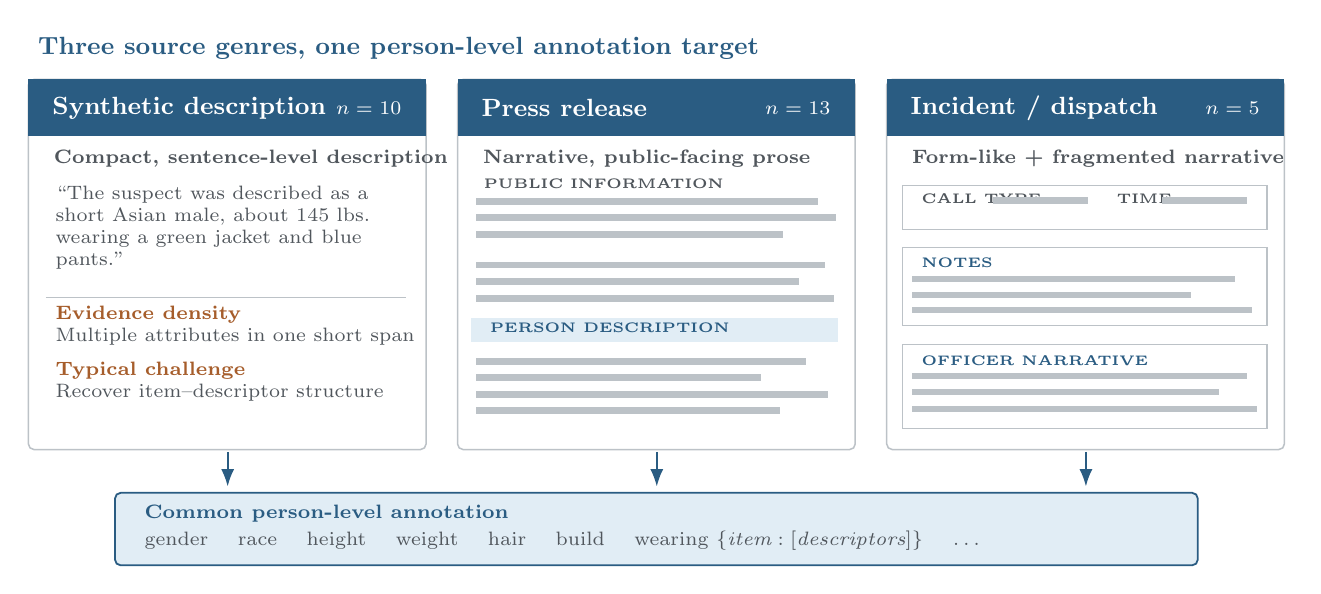
\begin{tikzpicture}[x=1cm,y=1cm,font=\sffamily]
  \definecolor{panelblue}{RGB}{42,92,130}
  \definecolor{panelblue2}{RGB}{225,237,245}
  \definecolor{panelgray}{RGB}{245,246,247}
  \definecolor{linegray}{RGB}{188,194,199}
  \definecolor{textgray}{RGB}{80,86,92}
  \definecolor{accent}{RGB}{166,93,43}

  % Overall title ribbon
  \node[anchor=west,font=\bfseries\small,text=panelblue] at (0,6.55)
    {Three source genres, one person-level annotation target};

  % ---------------- Synthetic panel ----------------
  \draw[rounded corners=2pt,line width=.55pt,draw=linegray,fill=white] (0,1.45) rectangle (5.05,6.15);
  \fill[panelblue] (0,5.43) rectangle (5.05,6.15);
  \node[anchor=west,text=white,font=\bfseries\small] at (.18,5.79) {Synthetic description};
  \node[anchor=east,text=white,font=\bfseries\scriptsize] at (4.86,5.79) {$n=10$};
  \node[anchor=west,font=\scriptsize\bfseries,text=textgray] at (.20,5.15) {Compact, sentence-level description};
  \node[anchor=north west,align=left,text width=4.55cm,font=\scriptsize,text=textgray]
    at (.22,4.92) {``The suspect was described as a short Asian male, about 145 lbs. wearing a green jacket and blue pants.''};
  \draw[draw=linegray,line width=.45pt] (.22,3.38) -- (4.80,3.38);
  \node[anchor=west,font=\scriptsize\bfseries,text=accent] at (.22,3.16) {Evidence density};
  \node[anchor=west,font=\scriptsize,text=textgray] at (.22,2.88) {Multiple attributes in one short span};
  \node[anchor=west,font=\scriptsize\bfseries,text=accent] at (.22,2.45) {Typical challenge};
  \node[anchor=west,font=\scriptsize,text=textgray] at (.22,2.17) {Recover item--descriptor structure};

  % ---------------- Press release panel ----------------
  \draw[rounded corners=2pt,line width=.55pt,draw=linegray,fill=white] (5.45,1.45) rectangle (10.50,6.15);
  \fill[panelblue] (5.45,5.43) rectangle (10.50,6.15);
  \node[anchor=west,text=white,font=\bfseries\small] at (5.63,5.79) {Press release};
  \node[anchor=east,text=white,font=\bfseries\scriptsize] at (10.31,5.79) {$n=13$};
  \node[anchor=west,font=\scriptsize\bfseries,text=textgray] at (5.65,5.15) {Narrative, public-facing prose};
  \node[anchor=west,font=\tiny\bfseries,text=textgray] at (5.66,4.82) {PUBLIC INFORMATION};
  % schematic narrative lines
  \foreach \y/\w in {4.56/4.35,4.35/4.58,4.14/3.90,3.75/4.43,3.54/4.10,3.33/4.55} {
    \fill[linegray] (5.68,\y) rectangle ++(\w,.085);
  }
  \fill[panelblue2] (5.62,2.82) rectangle (10.28,3.12);
  \node[anchor=west,font=\tiny\bfseries,text=panelblue] at (5.74,3.00) {PERSON DESCRIPTION};
  \foreach \y/\w in {2.53/4.20,2.32/3.62,2.11/4.48,1.90/3.86} {
    \fill[linegray] (5.68,\y) rectangle ++(\w,.085);
  }

  % ---------------- Dispatch panel ----------------
  \draw[rounded corners=2pt,line width=.55pt,draw=linegray,fill=white] (10.90,1.45) rectangle (15.95,6.15);
  \fill[panelblue] (10.90,5.43) rectangle (15.95,6.15);
  \node[anchor=west,text=white,font=\bfseries\small] at (11.08,5.79) {Incident / dispatch};
  \node[anchor=east,text=white,font=\bfseries\scriptsize] at (15.76,5.79) {$n=5$};
  \node[anchor=west,font=\scriptsize\bfseries,text=textgray] at (11.10,5.15) {Form-like + fragmented narrative};

  % small form fields
  \draw[draw=linegray,line width=.4pt] (11.10,4.80) rectangle (15.73,4.24);
  \node[anchor=west,font=\tiny\bfseries,text=textgray] at (11.22,4.64) {CALL TYPE};
  \fill[linegray] (12.25,4.57) rectangle (13.45,4.66);
  \node[anchor=west,font=\tiny\bfseries,text=textgray] at (13.70,4.64) {TIME};
  \fill[linegray] (14.40,4.57) rectangle (15.48,4.66);

  \draw[draw=linegray,line width=.4pt] (11.10,4.02) rectangle (15.73,3.02);
  \node[anchor=west,font=\tiny\bfseries,text=panelblue] at (11.22,3.82) {NOTES};
  \foreach \y/\w in {3.58/4.10,3.38/3.55,3.18/4.32} {
    \fill[linegray] (11.22,\y) rectangle ++(\w,.075);
  }

  \draw[draw=linegray,line width=.4pt] (11.10,2.78) rectangle (15.73,1.72);
  \node[anchor=west,font=\tiny\bfseries,text=panelblue] at (11.22,2.58) {OFFICER NARRATIVE};
  \foreach \y/\w in {2.35/4.25,2.14/3.90,1.93/4.38} {
    \fill[linegray] (11.22,\y) rectangle ++(\w,.075);
  }

  % arrows to common annotation target
  \draw[-{Latex[length=2.2mm]},line width=.7pt,draw=panelblue] (2.53,1.42) -- (2.53,.98);
  \draw[-{Latex[length=2.2mm]},line width=.7pt,draw=panelblue] (7.98,1.42) -- (7.98,.98);
  \draw[-{Latex[length=2.2mm]},line width=.7pt,draw=panelblue] (13.43,1.42) -- (13.43,.98);

  % common target box
  \draw[rounded corners=2pt,line width=.65pt,draw=panelblue,fill=panelblue2] (1.10,-.02) rectangle (14.85,.90);
  \node[anchor=west,font=\scriptsize\bfseries,text=panelblue] at (1.35,.63) {Common person-level annotation};
  \node[anchor=west,font=\scriptsize,text=textgray] at (1.35,.29)
    {gender \quad race \quad height \quad weight \quad hair \quad build \quad wearing $\{\textit{item}:[\textit{descriptors}]\}$ \quad $\ldots$};
\end{tikzpicture}
    \caption{Source heterogeneity in the 28-document proof-of-concept subset.
    The synthetic panel shows an actual corpus example. The press-release and
    incident/dispatch panels schematically represent the organization of those
    source types rather than reproducing potentially identifying source text.
    Despite these differences in genre and layout, all three source types map
    to the same person-level annotation schema.}
    \label{fig:source-heterogeneity}
\end{figure*}


\subsection{Person-Level Annotation}
\label{subsec:dataset-annotation}

Annotations are organized at the person level rather than only at the document
level. Each document identifier maps to an array of person records, which
allows a document to contain zero, one, or multiple annotated people without
merging their attributes. In the 28-document subset, six documents contain no
annotated person description, 21 contain one person record, and one document
contains two person records, yielding 23 person-level annotation records in
total.

Each person record contains a common structured schema covering demographic,
physical, behavioral, and appearance attributes. The schema includes
\texttt{gender}, \texttt{race}, \texttt{height}, \texttt{weight},
\texttt{hair\_color}, \texttt{tattoos}, \texttt{backpack},
\texttt{headphones}, \texttt{smoking}, \texttt{posture}, \texttt{vehicle},
\texttt{facial\_hair}, \texttt{hair\_length}, and \texttt{build}. Clothing is
represented by the nested \texttt{wearing} field. Rather than storing clothing
as a flat label, \texttt{wearing} maps each item to zero or more descriptors.
For example, a description containing a green jacket and blue pants is encoded
as \texttt{jacket:[green]} and \texttt{pants:[blue]}. This representation lets
the evaluation separately ask whether the clothing item itself was recovered
and whether its associated descriptors were recovered.

The present paper evaluates the four attribute groups with sufficient coverage
to support the proof-of-concept study: gender, race, height, and clothing.
Table~\ref{tab:attribute-coverage} reports their person-level gold coverage in
the 28-document subset. Gender is present in all 23 person records, race in 22,
clothing in 18, and height in 13. Other fields are considerably sparser in this
subset: weight appears in seven person records and hair color in six, while
each remaining populated field appears in at most three.

\begin{table}[t]
    \centering
    \caption{Gold annotation coverage for the attribute groups evaluated in the
    28-document proof-of-concept subset. Percentages use the 23 person-level
    annotation records as the denominator.}
    \label{tab:attribute-coverage}
    \begin{tabular}{lrr}
        \toprule
        Attribute group & Person records & Coverage \\
        \midrule
        Gender & 23 & 100.0\% \\
        Race & 22 & 95.7\% \\
        Height & 13 & 56.5\% \\
        Clothing (\texttt{wearing}) & 18 & 78.3\% \\
        \bottomrule
    \end{tabular}
\end{table}

Missing attributes are retained explicitly in the annotation structure rather
than interpreted as negative evidence. This is important for evaluation:
absence of a gold value means that the source text does not provide an
annotated value for that person, not that the corresponding physical or
demographic property is known to be absent.

\subsection{Proof-of-Concept Evaluation Set}
\label{subsec:dataset-poc}

Unless stated otherwise, the experiments in this paper use the 28
source-derived documents consisting of the \texttt{Synthetic},
\texttt{Press Release}, and \texttt{Incident Reports} subsets. We use this set
as a small proof of concept for structured attribute recovery across several
document styles. The generated subsets are not mixed into the reported
proof-of-concept results.

The evaluation preserves the person-level annotation structure. Consequently,
a system can be evaluated not only on whether an attribute appears somewhere
in a document, but also, where applicable, on whether the extracted attribute
is associated with the correct person record. The exact matching rules for
fixed attributes, clothing-item recovery, clothing descriptors, and
person-aware scoring are defined in Section~\ref{sec:experiments}.

\subsection{Provenance and Data Handling}
\label{subsec:dataset-provenance}

The 28 source-derived records were obtained from or through WLPD. The ten
synthetic descriptions were provided by WLPD; the incident/dispatch
records are historical WLPD records; and the press releases are public-facing
WLPD material. Identifying information in the historical incident-report
material was redacted before research use. The consolidated metadata preserves
the subset assignment, source path or lineage, and annotation linkage for each
indexed document; event metadata is retained where available. Preserving this
provenance is useful for reproducing the evaluation and for later analysis of
source- or genre-specific behavior rather than flattening all documents into a
single undifferentiated text collection.

The annotations represent attributes stated in the source text; \posid{} is
evaluated on recovering those textual descriptions rather than predicting
unobserved demographic or physical characteristics. The limitations of the
annotation schema, source reporting practices, and demographic vocabulary are
discussed separately in Section~\ref{sec:discussion}.


\section{\posid{} Method}
\label{sec:method}

\subsection{Problem Formulation and Overview}
\label{subsec:method-overview}

Let a document be an ordered sequence of sentences
$T=\langle s_1,\ldots,s_n\rangle$.  Given a small set of domain-relevant query
phrases $Q$ and a target attribute set $O$, the task is to recover a
person-indexed collection of structured attribute--value pairs from $T$.  In
this work,
\[
O=\{\textsc{gender},\textsc{race},\textsc{height},\textsc{clothing}\},
\]
where the first three attributes have constrained value forms and clothing is
open-vocabulary: both the item name and its descriptors may vary with the
text.

\posid{} decomposes this task into two stages (Figure~\ref{fig:posid-architecture}).
The first stage retrieves a small set of \emph{candidate sentences} that are
likely to contain relevant evidence.  The second stage performs structured
attribute extraction only over those candidates and then associates the
resulting mentions with person records.  This separation is intentional: a
selector answers \emph{where to look}, while the extraction layer decides
\emph{what structured facts are sufficiently supported by the local text}.
Different lexical or semantic selectors can therefore be compared without
changing the downstream extraction procedure.

\begin{figure*}[htbp]
    \centering
    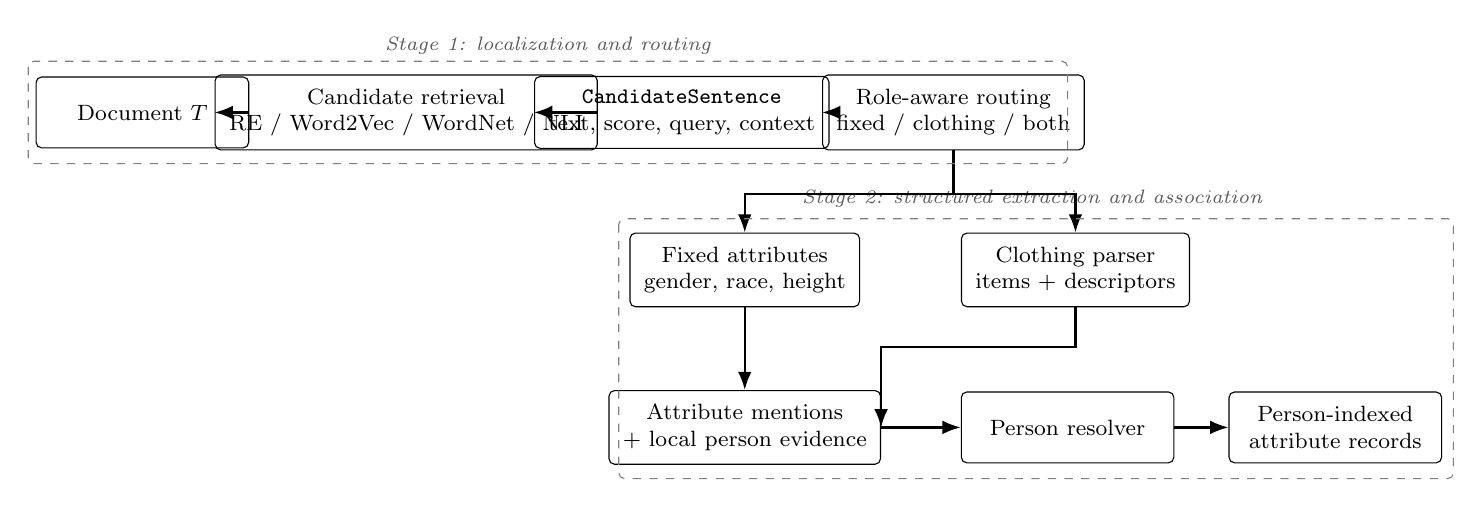
\begin{tikzpicture}[
        >=Latex,
        box/.style={draw, rounded corners=2pt, align=center, inner sep=5pt,
                    minimum height=9mm, minimum width=27mm, font=\footnotesize},
        arrow/.style={->, thick},
        stage/.style={font=\scriptsize\itshape, text=gray!70!black}
    ]
        % Stage 1: localization and routing
        \node[box] (doc) at (0,0) {Document $T$};
        \node[box] (retrieve) at (3.35,0) {Candidate retrieval\\RE / Word2Vec / WordNet / NLI};
        \node[box] (cand) at (6.85,0) {\texttt{CandidateSentence}\\text, score, query, context};
        \node[box] (route) at (10.30,0) {Role-aware routing\\fixed / clothing / both};
        \node[stage] at (5.15,0.85) {Stage 1: localization and routing};

        % Stage 2: extraction branches
        \node[box] (fixed) at (7.65,-2.0) {Fixed attributes\\gender, race, height};
        \node[box] (cloth) at (11.85,-2.0) {Clothing parser\\items + descriptors};
        \node[box] (mentions) at (7.65,-4.0) {Attribute mentions\\+ local person evidence};
        \node[box] (resolve) at (11.75,-4.0) {Person resolver};
        \node[box] (output) at (15.15,-4.0) {Person-indexed\\attribute records};
        \node[stage] at (11.30,-1.10) {Stage 2: structured extraction and association};

        \draw[arrow] (doc) -- (retrieve);
        \draw[arrow] (retrieve) -- (cand);
        \draw[arrow] (cand) -- (route);
        \draw[arrow] (route.south) -- ++(0,-0.55) -| (fixed.north);
        \draw[arrow] (route.south) -- ++(0,-0.55) -| (cloth.north);
        \draw[arrow] (fixed.south) -- (mentions.north);
        \draw[arrow] (cloth.south) -- ++(0,-0.5) -| (mentions.east);
        \draw[arrow] (mentions) -- (resolve);
        \draw[arrow] (resolve) -- (output);

        \draw[dashed, rounded corners=2pt, gray]
            (-1.45,0.65) rectangle (11.75,-0.65);
        \draw[dashed, rounded corners=2pt, gray]
            (6.05,-1.35) rectangle (16.65,-4.65);
    \end{tikzpicture}
    \caption{\posid{} separates candidate localization from structured
    extraction. Candidate provenance determines which extraction operations
    are valid for a candidate, while the final resolver associates extracted
    mentions with person records.}
    \Description{Two-stage POSID architecture. A document passes through candidate retrieval, a provenance-bearing CandidateSentence interface, and role-aware routing. Fixed-attribute and clothing extraction produce local attribute mentions, which are associated with person records by a resolver.}
    \label{fig:posid-architecture}
\end{figure*}

\subsection{Candidate Representation}
\label{subsec:candidate-representation}

Every selector returns the same provenance-bearing representation
\[
c=\langle i, x, r, q, \kappa\rangle,
\]
where $i$ is the sentence index, $x$ is the text returned by the selector,
$r$ is its relevance score, $q$ is the query or pattern responsible for the
selection, and $\kappa$ is the complete sentence or expanded local context.
This representation is important because the selectors do not return exactly
the same text.  A regular-expression selector may return only the matched
substring, whereas semantic selectors return the complete qualifying sentence.
Keeping $x$ and $\kappa$ separately allows the extractor to preserve the
selector's actual evidence while still recovering the context required for
attribute association.

For sentence fragments beginning with a form of \emph{wear} (e.g.,
``wearing a blue jacket''), the immediately preceding sentence is attached to
$\kappa$ when it contains an explicit person-role anchor such as
\emph{suspect}, \emph{victim}, or \emph{juvenile}.  This handles a common
fragmentation pattern in which the person is introduced in one sentence and
the clothing description begins in the next.

\subsection{Candidate Selectors}
\label{subsec:candidate-selectors}

The candidate stage is implemented through a common selector interface.  The
four selectors used in this study differ in how they score a sentence and in
how many candidates they return (Table~\ref{tab:selector-semantics}).  Let
$\operatorname{tok}(s)$ denote the tokens of sentence $s$.

\begin{table*}[t]
    \centering
    \caption{Candidate-selector semantics used by \posid{}.  Semantic
    selectors return the first sentence that satisfies their threshold in the
    current implementation; RE can return multiple matched sentences.}
    \label{tab:selector-semantics}
    \begin{tabular}{p{2.2cm}p{6.3cm}p{3.0cm}p{3.2cm}}
        \toprule
        Selector & Relevance criterion & Returned text & Candidate cardinality \\
        \midrule
        RE & Literal or explicit regular-expression match & Matched substring with full sentence in context & All matching sentences \\
        Word2Vec & Maximum token--query cosine similarity & Full sentence & First qualifying sentence \\
        WordNet & Noun-synset Wu--Palmer similarity & Full sentence & First qualifying sentence \\
        Zero-shot NLI & Query-conditioned NLI label score & Full sentence & First qualifying sentence \\
        \bottomrule
    \end{tabular}
\end{table*}

\paragraph{Pattern matching.}
For a query $q$, the RE selector uses exact lexical or regular-expression
matching.  Its relevance score is binary,
\[
R_{\mathrm{RE}}(s,q)=
\begin{cases}
1,& q\text{ matches }s,\\
0,& \text{otherwise.}
\end{cases}
\]
Queries are checked in a fixed order and each sentence is emitted at most once;
the first matching query becomes the candidate provenance $q$.  This ordering
is used later to distinguish candidates that can support clothing extraction
from candidates intended only for fixed attributes.

\paragraph{Word2Vec similarity.}
For Word2Vec~\cite{mikolov2013efficient}, candidate relevance is the strongest
similarity between a sentence token and a query:
\begin{equation}
R_{\mathrm{W2V}}(s,q)
=\max_{w\in\operatorname{tok}(s)}
\frac{\mathbf{v}_w^\top\mathbf{v}_q}
{\lVert\mathbf{v}_w\rVert\lVert\mathbf{v}_q\rVert}.
\label{eq:w2v-score}
\end{equation}
For multiple queries, the highest qualifying token--query pair supplies the
candidate score and provenance.  Tokens absent from the pretrained vocabulary
are ignored.

\paragraph{WordNet similarity.}
WordNet~\cite{wordnet98} provides a lexical alternative to distributional
embeddings.  Noun senses are compared with Wu--Palmer similarity.  In the
configuration evaluated here, each query is represented by its first noun
synset; sentence tokens are scanned in textual order and compared over their
noun synsets.  A sentence becomes a candidate when the first token--synset pair
meeting the configured threshold is encountered.  Thus the selector uses
lexical-semantic proximity while retaining deterministic first-hit behavior.

\paragraph{Zero-shot NLI.}
The fourth selector reformulates candidate retrieval as zero-shot text
classification using a pretrained natural-language-inference model\cite{yin2019benchmarking}.  A
sentence $s$ is the premise and each query $q$ is inserted into the hypothesis
\begin{equation}
h(q)=\text{``This example is }q\text{.''}
\label{eq:nli-template}
\end{equation}
The classifier's returned score for $q$ is used as
$R_{\mathrm{NLI}}(s,q)$.  The highest-scoring query above the configured
threshold supplies the candidate provenance.  No \incitext{} examples are used
to train or fine-tune this selector; the pretrained NLI model is used in a
zero-shot configuration.  The exact checkpoint and thresholds are reported in
Section~\ref{sec:experiments}.

\subsection{Routed Candidate Selection}
\label{subsec:stacked-routing}

A central design choice is that combining selectors does not mean taking their
unconditional union.  The routed configuration first applies the high-precision
RE selector using two query roles: a clothing cue based on \emph{wearing} and a
fixed-attribute pattern that localizes a suspect description.  Let $W$ denote
RE candidates produced by the clothing cue and $F$ the remaining RE candidates.
A semantic selector $M$ is invoked with the query \emph{clothes} only when no
clothing RE candidate is available:
\begin{equation}
C = F \cup
\begin{cases}
W, & W\neq\varnothing,\\
M(T,\{\text{clothes}\}), & W=\varnothing.
\end{cases}
\label{eq:stacked-routing}
\end{equation}
The semantic fallback can therefore recover an implicit clothing description
without adding semantic candidates when the explicit cue already localized the
relevant text.

Candidate provenance also controls downstream scope.  A candidate produced by
\emph{wearing} is allowed to contribute both fixed attributes and clothing; a
semantic \emph{clothes} candidate contributes clothing only; and the
fixed-attribute RE candidate contributes gender, race, and height only.  Since
the same sentence can legitimately enter through different roles, duplicate
work is removed using the tuple
$(i,x,b_f,b_c)$, where $b_f$ and $b_c$ indicate whether fixed and clothing
extraction are enabled.  Two identical sentence strings are therefore not
collapsed when they represent different extraction roles.

Algorithm~\ref{alg:posid} summarizes the routed pipeline.  Standalone selector
experiments use the same extraction stage but populate $C$ directly from the
corresponding selector rather than applying the fallback rule in
Equation~\ref{eq:stacked-routing}.

\begin{algorithm}[t]
\caption{Candidate routing and structured \posid{} recovery}
\label{alg:posid}
\KwIn{document $T$; RE selector $R$; optional semantic selector $M$; parser mode $\tau$}
\KwOut{person-indexed structured attributes $\widehat{A}$}
$C_R \leftarrow R(T,\{q_{\mathrm{wear}},q_{\mathrm{fixed}}\})$\;
$W \leftarrow \{c\in C_R : c.q=q_{\mathrm{wear}}\}$\;
$F \leftarrow C_R\setminus W$\;
\eIf{$W\neq\varnothing$}{
    $C\leftarrow F\cup W$\;
}{
    $C\leftarrow F\cup M(T,\{\text{clothes}\})$\;
}
construct sentence-level person anchors, prior-anchor context, and shared-anchor context\;
$L\leftarrow\varnothing$; $K\leftarrow\varnothing$ \tcp*{mentions and processed-role keys}
\ForEach{$c\in C$}{
    $(b_f,b_c)\leftarrow\operatorname{Role}(c.q)$\;
    $u\leftarrow\operatorname{Context}(c,T)$\;
    $k\leftarrow(c.i,u,b_f,b_c)$\;
    \If{$k\in K$}{continue\;}
    $K\leftarrow K\cup\{k\}$\;
    \If{$b_f$}{
        $L_f\leftarrow\operatorname{Fixed}(u)$\;
        $L\leftarrow L\cup L_f$\;
        \If{$L_f$ contains no height and the next sentence exists}{
            $L\leftarrow L\cup\operatorname{HeightOnly}(s_{c.i+1})$\;
        }
    }
    \If{$b_c$}{
        $L\leftarrow L\cup\operatorname{ClothingParser}(u,\tau)$\; \tcp*{Algorithm~\ref{alg:clothing}}
    }
}
$\widehat{A}\leftarrow\operatorname{ResolvePeople}(L)$\;
\Return $\widehat{A}$\;
\end{algorithm}

\subsection{Structured Extraction of Fixed Attributes}
\label{subsec:fixed-extraction}

Fixed attributes are extracted only from candidates whose provenance enables
fixed-attribute processing.  The extractor records an attribute mention with
its sentence index, character position, and nearest local person anchor so that
association can be resolved after all candidate evidence has been processed.

\paragraph{Gender.}
Gender is recognized through explicit whole-word lexical forms.  The current
mapping normalizes \emph{male}, \emph{man}, and \emph{boy} to \texttt{male},
and \emph{female}, \emph{woman}, and \emph{girl} to \texttt{female}.  The
system extracts only what is explicitly stated; it does not infer gender from a
name.

\paragraph{Race.}
Race is extracted from explicit race--gender adjacency rather than from an
isolated demographic token.  For the race vocabulary
\[
\{\text{asian, black, white, hispanic, latino, latina, indian}\},
\]
the extractor accepts both orders, $\langle\text{race},\text{gender}\rangle$
and $\langle\text{gender},\text{race}\rangle$.  Thus phrases such as
``Asian male'' and ``male Asian'' support the same race value.  Requiring the
local gender relation also prevents a color-like token occurring later in a
clothing description from being interpreted as race.

\paragraph{Height.}
Numeric height expressions are recognized with patterns covering forms such as
``6 feet 2 inches tall'', ``6-foot'', ``6 ft'', and ``5'10\textquotedbl''.
Qualitative \emph{short}/\emph{tall} is accepted only when it participates in a
demographic construction containing gender, optionally with an intervening race
term.  This prevents expressions such as ``short hair'' or ``tall building''
from becoming height values.  When a fixed-attribute candidate contains no
height, \posid{} additionally inspects the immediately following sentence and
retains only height mentions from that sentence.  Person anchors are resolved
normally, so height evidence attached to another explicitly named person is
not reassigned to the current person.

\subsection{Open-Vocabulary Clothing Extraction}
\label{subsec:clothing-extraction}

Clothing is treated differently because the set of possible item names and
modifiers is not closed.  For each clothing-enabled candidate, \posid{} first
defines the text span to parse.  If a form of \emph{wear} is present, the span
begins at that cue and continues through the remainder of the sentence.  If no
wear cue is present---as can occur for a semantic fallback candidate---the
extractor removes spans already identified as gender, race, or height and parses
the remaining candidate text.  This keeps the candidate selector responsible
for localization while allowing implicit clothing constructions such as a list
of apparel items without the word \emph{wearing}.

The selected span is tokenized and part-of-speech tagged with NLTK
\cite{nltk2002}.  The parser maintains a descriptor buffer $D$ and a current
noun run $N$.  Its principal rules are:
\begin{enumerate}[leftmargin=*,itemsep=2pt,topsep=3pt]
    \item adjective tokens are accumulated as descriptors;
    \item noun tokens form open-vocabulary clothing item names, with consecutive
    nouns merged into compounds such as \emph{tank top} or \emph{dress pants};
    \item a noun that is semantically close to the WordNet noun sense of
    \emph{color} is treated as a descriptor rather than an item name, providing
    a safeguard for colors that are mistagged as nouns;
    \item contextual modifiers such as \emph{dark} and \emph{light} are retained
    as descriptors when they modify a following noun; and
    \item compound pre-nominal forms such as ``buttoned up shirt'' preserve the
    verb/particle modifier as a descriptor of the following clothing noun.
\end{enumerate}
The resulting clothing fact is represented as
$\langle\textit{item},D\rangle$.  Surface forms are retained rather than mapped
to a fixed clothing ontology, and slash-separated item expressions are
normalized into separate item records before output.

Unexpected POS patterns create a precision--recall decision.  In the main
parser, once clothing extraction has begun, an otherwise-unhandled POS pattern
terminates the clothing scan.  This conservative rule prevents candidate
relevance from being treated as permission to consume arbitrarily distant
nouns after the local syntactic evidence has become unreliable.  A permissive
continuation mode instead closes the current noun run and continues scanning,
which can recover a later clothing mention at the risk of additional false
positives.  We retain continuation as an explicit ablation and evaluate the
tradeoff in Section~\ref{sec:results}.

Algorithm~\ref{alg:clothing} makes the open-vocabulary parser explicit.  The
procedure keeps the candidate-selection decision outside the parser: by the
time it is called, the input has already been localized as clothing evidence.
Within that evidence, the parser incrementally constructs item names and
associated descriptors and decides whether syntactically unexpected material
should merely close the current item or terminate the scan.

\begin{algorithm}[t]
\caption{Open-vocabulary clothing parser}
\label{alg:clothing}
\KwIn{candidate context $u$; parser mode $\tau\in\{\textsc{continue},\textsc{stop}\}$}
\KwOut{clothing facts $S=\{\langle item,D\rangle\}$}
$p\leftarrow\operatorname{WearSpan}(u)$\;
\eIf{$p\neq\varnothing$}{
    $x\leftarrow p$\;
}{
    $x\leftarrow\operatorname{RemoveFixedSpans}(u)$\;
}
$(w_1,t_1),\ldots,(w_m,t_m)\leftarrow\operatorname{POSTag}(\operatorname{Tokenize}(x))$\;
$S\leftarrow\varnothing$; $D\leftarrow[\ ]$; $N\leftarrow[\ ]$\;
\SetKwFunction{Flush}{FLUSH}
\SetKwProg{Fn}{Function}{:}{end}
\Fn{\Flush{}}{
    \If{$N\neq[\ ]$}{
        $item\leftarrow\operatorname{Join}(N)$\;
        \ForEach{$z\in\operatorname{SplitSlash}(item)$}{
            $S\leftarrow S\cup\{\langle z,D\rangle\}$\;
        }
    }
    $D\leftarrow[\ ]$; $N\leftarrow[\ ]$\;
}
\For{$j\leftarrow1$ \KwTo $m$}{
    $w\leftarrow\operatorname{casefold}(w_j)$; $t\leftarrow t_j$\;
    \If{$t\in\{\mathrm{VBD},\mathrm{VBN}\}$ and $t_{j+1}\in\{\mathrm{RP},\mathrm{RB}\}$ and $t_{j+2}$ is noun}{
        append $w\,w_{j+1}$ to $D$; continue\;
    }
    \If{$t\in\{\mathrm{RP},\mathrm{RB}\}$ and the previous token was consumed as a compound modifier}{continue\;}
    \If{$w$ is a boundary, \emph{both}, or \emph{but}}{\Flush{}; continue\;}
    \If{$t$ is adjective, or $w\in\{\text{dark},\text{light}\}$ before a noun}{append $w$ to $D$; continue\;}
    \If{$t$ is noun}{
        \If{$w$ is a person anchor or ignored scaffold word}{\Flush{}; continue\;}
        \If{$\operatorname{ColorSim}(w)>\theta_{color}$}{\Flush{}; append $w$ to $D$; continue\;}
        append $w$ to $N$ \tcp*{consecutive nouns form compound item names}
        continue\;
    }
    \If{$t$ is determiner, conjunction, preposition, punctuation, or delimiter}{\Flush{}; continue\;}
    \If{$\tau=\textsc{stop}$ and parsing has begun}{break\;}
    \Flush{} \tcp*{continue mode closes the current item and keeps scanning}
}
\Flush{}\;
\Return $S$\;
\end{algorithm}

\subsection{Person Association and Mention Resolution}
\label{subsec:person-resolution}

Attribute extraction and person association are separated.  Before candidates
are processed, \posid{} scans the document for narrow person anchors: explicit
roles (\emph{suspect}, \emph{victim}, and \emph{juvenile}) and capitalized
name-like tokens after excluding demographic and role stopwords.  Anchors that
occur inside the clothing portion of a sentence are not treated as person
names, reducing collisions between apparel/color terms and person evidence.

Each extracted mention is first linked to the nearest preceding
anchor in the same local context.  The resolver then processes mentions in
textual order and maintains the most recently active person records.  Explicit
anchors take precedence.  When no explicit local anchor is available, pronoun cues
(\emph{he}, \emph{she}, or \emph{they}) carry recent person context into
resolution.  The resolver can use already extracted gender to prefer a
compatible recent person for \emph{he} or \emph{she}; this is only an
association constraint and never creates a new gender value.  If a sentence
introduces multiple anchors in a coordinated construction and a subsequent
clothing sentence uses \emph{both}, the clothing mention is copied to those
shared anchors.  Otherwise an unanchored mention is assigned to the nearest
active local person, or to a deterministic anonymous person record if no person
context exists.

The final output is a list of person records for each document.  Fixed
attributes are stored as scalar values, while clothing is stored as a list of
item--descriptor structures.  This person-indexed representation supports both
document-level extraction metrics and the stricter person-aware diagnostic
defined in Section~\ref{sec:experiments}.


\section{Experimental Protocol}
\label{sec:experiments}

The experiments are designed to evaluate the two decisions separated by
\posid{}: candidate localization and structured extraction.  We first compare
lexical and semantic candidate selectors while holding the downstream
extractor fixed.  We then report attribute-level extraction for the selected
routed configuration.  Finally, we isolate the clothing parser's behavior when
local syntactic evidence becomes unreliable by comparing continued scanning
against conservative early termination.

\subsection{Evaluation Corpus}
\label{subsec:experimental-corpus}

All experiments in this paper use the 28-document source-derived subset defined
in Section~\ref{subsec:dataset-poc}: 10 synthetic descriptions, 13 press
releases, and 5 incident/dispatch records.  The subset contains 23 gold
person-annotation records distributed across 22 documents; six documents
contain no annotated person description and therefore also test whether a
method introduces unsupported extractions.  The gold annotations contain 23
gender values, 22 race values, and 13 height values.  Clothing is represented
as item--descriptor structures as described in
Section~\ref{subsec:dataset-annotation}.

Because \posid{} performs no target-task parameter learning, we do not create a
supervised train/test split for this proof-of-concept study.  Every method is
run over the same 28 documents using the frozen selector queries, thresholds,
and extraction rules listed below.  The generated portions of \incitext{} are
not included in the results reported in this paper.

\subsection{Compared Candidate-Selection Configurations}
\label{subsec:experimental-methods}

We evaluate four individual candidate selectors and two routed combinations.
In every case, the selected candidate is passed to the same \posid{} structured
extraction layer; the experiment therefore changes \emph{where the extractor
looks}, not the attribute extraction rules themselves.  Table~\ref{tab:selector-config}
summarizes the frozen configuration.

\begin{table*}[t]
    \centering
    \caption{Candidate-selection configurations used in the proof-of-concept
    experiments.  RE returns all matching sentences (at most one candidate per
    sentence); the semantic selectors return the first sentence satisfying the
    configured threshold.}
    \label{tab:selector-config}
    \small
    \begin{tabular}{p{0.18\textwidth}p{0.25\textwidth}p{0.13\textwidth}p{0.34\textwidth}}
        \toprule
        Configuration & Query / evidence & Threshold & Selection or routing behavior \\
        \midrule
        RE + \posid{} & \texttt{wearing}; fixed suspect pattern & exact match & All matching sentences; \texttt{wearing} is evaluated before the fixed pattern. \\
        Word2Vec + \posid{} & \texttt{clothes} & $\geq 0.50$ & First sentence whose best token--query cosine similarity qualifies. \\
        WordNet + \posid{} & \texttt{clothes} & $\geq 0.90$ & First qualifying sentence using Wu--Palmer noun-synset similarity. \\
        Zero-shot NLI + \posid{} & \texttt{clothes} & $>0.85$ & First sentence whose zero-shot label score qualifies. \\
        RE + WordNet + \posid{} & RE primary; \texttt{clothes} fallback & as above & Use RE clothing candidates when present; otherwise invoke WordNet for clothing. \\
        RE + NLI + \posid{} & RE primary; \texttt{clothes} fallback & as above & Use RE clothing candidates when present; otherwise invoke zero-shot NLI for clothing. \\
        \bottomrule
    \end{tabular}
\end{table*}

The RE selector is supplied two queries in a fixed order.  The first is the
literal cue \texttt{wearing}.  The second is the fixed-attribute candidate
pattern
\begin{center}
\texttt{\detokenize{[^.]*suspect.*male[^.]*\.}}
\end{center}
with case-insensitive matching.  Query order is deliberate because a sentence
matching both patterns is labeled by the first matching query and can therefore
be routed as a clothing-bearing candidate while still permitting fixed
attribute extraction.  The routed methods retain fixed-attribute RE candidates
regardless of whether the clothing path uses the RE candidate or the semantic
fallback.

The Word2Vec selector uses the pruned \texttt{word2vec\_sample} vectors
available through NLTK.  The WordNet selector represents \texttt{clothes} by
its first noun synset and compares it against noun synsets of sentence tokens
using Wu--Palmer similarity.  The zero-shot selector uses
\texttt{facebook/bart-large-mnli} through the Hugging Face
\texttt{zero-shot-classification} pipeline with \texttt{multi\_label=False}.
For every sentence, the candidate label is inserted into the explicit
hypothesis template
\begin{equation}
\texttt{This example is \{\}.}
\label{eq:experiment-nli-template}
\end{equation}
including the terminal period.  No target-corpus examples are used to train or
fine-tune the NLI model.

\subsection{Extraction Configuration}
\label{subsec:experimental-extraction}

All candidate-selection conditions use the same \posid{} extractor described
in Section~\ref{sec:method}.  Sentence and word tokenization use NLTK, and
clothing parsing uses the averaged-perceptron POS tagger.  The WordNet
color-sense safeguard treats a noun token as a color descriptor when its
Wu--Palmer similarity to the first noun sense of \emph{color} exceeds $0.70$.
Gender, race, numeric/relative height, next-sentence height recovery, compound
clothing handling, slash-separated item handling, role-aware candidate
processing, and person association are otherwise fixed across experimental
conditions.

The main parser configuration sets
\texttt{stop\_on\_unexpected\_pos=True}.  Once clothing parsing has begun, the
first otherwise-unhandled POS token terminates the clothing scan.  The
controlled ablation changes only this flag to \texttt{False}: the current noun
run is closed, but scanning continues and may recover a later item.  The
candidate selector, fixed-attribute rules, color threshold, tagging model,
person-resolution logic, and all other parser behavior are held constant.  The
comparison therefore isolates the precision--recall effect of syntactic
termination rather than replacing the parser with a different implementation.

\subsection{Primary Evaluation Metrics}
\label{subsec:experimental-metrics}

We report micro-aggregated precision, recall, and $F_1$ from counts accumulated
across the evaluation documents:
\begin{equation}
P=\frac{TP}{TP+FP},\qquad
R=\frac{TP}{TP+FN},\qquad
F_1=\frac{2PR}{P+R}.
\label{eq:prf}
\end{equation}
All textual values are compared after case folding and whitespace
normalization.  Height surfaces additionally undergo format normalization so
that equivalent representations are compared consistently.

\paragraph{Fixed attributes.}
For gender, race, and height, gold and predicted values are pooled within each
document and compared by exact one-to-one multiset matching after
normalization.  A matched value contributes one true positive; unmatched
predictions and gold values contribute false positives and false negatives,
respectively.  Document-level counts are then summed before computing the
corpus-level scores.  This evaluation does not give credit for predicting an
attribute that is not explicitly present in the gold annotation.

\paragraph{Clothing Attr-Only.}
Attr-Only evaluates recovery of clothing item names independently of their
descriptors.  Clothing instances are grouped by normalized item name and
matched one-to-one within each document.  A matched item contributes one true
positive, while unmatched predicted and gold items contribute false positives
and false negatives.

\paragraph{Clothing Attr-Value.}
Attr-Value evaluates the richer item--descriptor structure.  Same-name clothing
instances are paired one-to-one, choosing the pairing that maximizes descriptor
overlap when duplicate item names occur.  For each matched pair, the item name
contributes one true-positive unit and every correctly recovered descriptor
contributes an additional true-positive unit.  Missing gold descriptors and
extra predicted descriptors contribute false-negative and false-positive units.
An entirely unmatched clothing item contributes one item unit plus its
associated descriptor units to the corresponding error count.  This metric
therefore distinguishes partial descriptor recovery from an all-or-nothing
item match.

\subsection{Person-Aware Diagnostic}
\label{subsec:person-aware-metric}

The primary metrics above measure whether the correct structured facts are
recovered within each document.  We additionally compute a stricter
person-aware diagnostic to expose attribute-association errors.  Gold and
predicted people are paired deterministically, preferring an exact person ID,
then an explicit matching role; singleton documents are paired directly.  If
multiple unresolved people remain, the pairing uses overlap in already
extracted gender, race, height, and clothing-item evidence, with ambiguous ties
recorded separately.  Fixed attributes are then scored only within the matched
person pair.  For clothing, Attr-Only requires a matching item name within the
person pair, while the strict person-aware Attr-Value diagnostic requires the
matched item's descriptor set to agree exactly.

Because the present 28-document subset contains only one multi-person document,
person-aware scores are treated as a diagnostic rather than evidence of broad
multi-person generalization.

\subsection{Reproducibility Configuration}
\label{subsec:experimental-reproducibility}

The frozen runs use Python~3.9 with NLTK~3.9.2, gensim~4.4.0,
NumPy~1.26.4, and SciPy~1.13.1.  The zero-shot path uses
PyTorch~2.2.2 and Transformers~4.44.2 with the
\texttt{facebook/bart-large-mnli} checkpoint cached locally.  The required
NLTK resources are WordNet, \texttt{averaged\_perceptron\_tagger\_eng}, and
\texttt{word2vec\_sample}.  No model training or stochastic generation is
performed during evaluation; every configuration operates on the same indexed
document set and writes document-level predictions before metric computation.

\section{Results and Analysis}
\label{sec:results}

We first report the frozen candidate-selection results with conservative early
termination as the main clothing-parser configuration.  We then examine
precision and recall in more detail and use permissive continuation as a
single-factor ablation.  All results use the same 28-document proof-of-concept
subset and the frozen settings in Section~\ref{sec:experiments}.

\subsection{Candidate Selection and Attribute Recovery}
\label{subsec:results-main}

Table~\ref{tab:main-results} gives the overall $F_1$ view.  The standalone
Word2Vec, WordNet, and NLI selectors are configured only with the query
\texttt{clothes}; fixed-attribute extraction is therefore outside their
configured retrieval scope.  We denote those cells by ``--'' rather than zero,
because they are not attempted fixed-attribute conditions.  RE-containing
configurations expose the fixed-attribute candidate role in addition to the
clothing path.

\begin{table*}[t]
    \centering
    \caption{Primary $F_1$ results on the 28-document proof-of-concept subset
    with conservative early termination as the main clothing parser.  ``--''
    indicates that the standalone semantic selector was configured for
    clothing retrieval only, so fixed attributes are not applicable under that
    configuration.}
    \label{tab:main-results}
    \small
    \setlength{\tabcolsep}{8pt}
    \begin{tabular}{lccccc}
        \toprule
        Method & Gender & Race & Height & Clothing AO & Clothing AV \\
        \midrule
        RE + \posid{} & .789 & .811 & .818 & .795 & .830 \\
        Word2Vec + \posid{} & -- & -- & -- & .529 & .540 \\
        WordNet + \posid{} & -- & -- & -- & .414 & .400 \\
        Zero-shot NLI + \posid{} & -- & -- & -- & .741 & .768 \\
        RE + WordNet + \posid{} & .789 & .811 & .818 & \textbf{.824} & \textbf{.857} \\
        RE + NLI + \posid{} & .789 & .811 & .818 & .814 & .852 \\
        \bottomrule
    \end{tabular}
\end{table*}

The fixed-attribute results are identical for RE, RE + WordNet, and RE + NLI
because the semantic fallback is restricted to clothing retrieval.  Rather than
repeat the same precision/recall triplets for all three configurations,
Table~\ref{tab:fixed-detail} reports them once.  Precision is 1.0 for gender,
race, and height, while recall is lower, indicating conservative fixed-attribute
rules that avoid false positives on this subset but leave some annotated values
unrecovered.

\begin{table}[t]
    \centering
    \caption{Fixed-attribute performance for all RE-containing configurations.
    The values are identical because semantic fallback changes only the
    clothing-retrieval path.}
    \label{tab:fixed-detail}
    \small
    \begin{tabular}{lrrr}
        \toprule
        Attribute & Precision & Recall & $F_1$ \\
        \midrule
        Gender & 1.000 & .652 & .789 \\
        Race & 1.000 & .682 & .811 \\
        Height & 1.000 & .692 & .818 \\
        \bottomrule
    \end{tabular}
\end{table}

Clothing recovery is more sensitive to candidate selection.  The detailed
precision--recall values in Table~\ref{tab:clothing-detail} show that RE +
WordNet obtains the highest main-configuration $F_1$ on both Attr-Only (.824)
and Attr-Value (.857), with RE + NLI close behind (.814/.852).  Standalone NLI
is substantially more balanced than Word2Vec or WordNet, while standalone
WordNet is precise when it fires but strongly recall-limited.  These different
retrieval profiles feed the same downstream POSID extractor, illustrating why
candidate localization and structured extraction are treated as separate
components.

\begin{table*}[t]
    \centering
    \caption{Detailed clothing extraction results for the main conservative
    parser.  AO denotes Attr-Only and AV denotes Attr-Value.}
    \label{tab:clothing-detail}
    \small
    \setlength{\tabcolsep}{6pt}
    \begin{tabular}{lrrrrrr}
        \toprule
        & \multicolumn{3}{c}{Attr-Only} & \multicolumn{3}{c}{Attr-Value} \\
        \cmidrule(lr){2-4}\cmidrule(lr){5-7}
        Method & P & R & $F_1$ & P & R & $F_1$ \\
        \midrule
        Word2Vec + \posid{} & .750 & .409 & .529 & .841 & .398 & .540 \\
        RE + \posid{} & .846 & .750 & .795 & .910 & .763 & .830 \\
        WordNet + \posid{} & .857 & .273 & .414 & .889 & .258 & .400 \\
        Zero-shot NLI + \posid{} & .811 & .682 & .741 & .887 & .677 & .768 \\
        RE + WordNet + \posid{} & .854 & .795 & \textbf{.824} & .915 & .806 & \textbf{.857} \\
        RE + NLI + \posid{} & .833 & .795 & .814 & .904 & .806 & .852 \\
        \bottomrule
    \end{tabular}
\end{table*}

\subsection{Continuation Ablation}
\label{subsec:results-early-stop}

The main parser terminates once clothing extraction has begun and local POS
evidence becomes unsupported.  Table~\ref{tab:early-stop-ablation} asks what
happens if this decision is reversed and scanning is allowed to continue.  The
ablation changes only this parser flag; fixed-attribute scores are therefore
unchanged.

\begin{table*}[t]
    \centering
    \caption{Main conservative parser versus permissive continuation.  $\Delta$
    is main $F_1$ minus continuation $F_1$; positive values favor conservative
    termination.}
    \label{tab:early-stop-ablation}
    \small
    \begin{tabular}{lrrrrrr}
        \toprule
        & \multicolumn{3}{c}{Attr-Only $F_1$} & \multicolumn{3}{c}{Attr-Value $F_1$} \\
        \cmidrule(lr){2-4}\cmidrule(lr){5-7}
        Method & Main stop & Continue & $\Delta$ & Main stop & Continue & $\Delta$ \\
        \midrule
        Word2Vec + \posid{} & .529 & .535 & -.006 & .540 & .549 & -.009 \\
        RE + \posid{} & .795 & .761 & +.034 & .830 & .813 & +.017 \\
        WordNet + \posid{} & .414 & .426 & -.012 & .400 & .416 & -.016 \\
        Zero-shot NLI + \posid{} & .741 & .719 & +.022 & .768 & .759 & +.009 \\
        RE + WordNet + \posid{} & .824 & .787 & +.037 & \textbf{.857} & .839 & +.018 \\
        RE + NLI + \posid{} & .814 & .747 & \textbf{+.067} & .852 & .817 & \textbf{+.035} \\
        \bottomrule
    \end{tabular}
\end{table*}

The largest effect occurs for RE + NLI.  Attr-Only precision rises from .673
under continuation to .833 under the main stopping rule, while recall changes
from .841 to .795; $F_1$ consequently increases from .747 to .814.  Attr-Value
shows the same pattern: precision increases from .796 to .904 while recall
changes from .839 to .806, raising $F_1$ from .817 to .852.  RE and RE +
WordNet also improve under conservative termination, as does standalone NLI.

The direction reverses slightly for standalone Word2Vec and WordNet.  This
qualifies the result: stopping is not intrinsically superior for every
retriever.  Rather, it behaves as a precision-control rule when candidate
localization has already placed POSID in a strongly relevant region.  Permissive
continuation can retain useful later evidence for weaker or sparse candidate
selectors, but it can also admit unrelated nouns after the local syntactic
signal has deteriorated.  On this proof-of-concept set, the conservative policy
provides the stronger tradeoff for the RE-based routed configurations used as
the principal POSID setting.

\subsection{Person-Aware Diagnostic}
\label{subsec:results-person-aware}

The evaluation protocol also defines a stricter person-aware diagnostic, but we
do not mix its previously generated permissive-parser numbers into the main
conservative-parser results.  A person-aware rerun under the frozen main parser
is required before reporting those values.  This omission does not affect the
primary document-level metrics above.  Moreover, the present subset contains
only one multi-person document, so any person-aware result from these 28
documents should in any case be interpreted as a diagnostic rather than as
evidence of broad multi-person attribution capability.

\section{Discussion and Limitations}
\label{sec:discussion}

\subsection{Discussion}
\label{subsec:discussion}

The experiments support a modular view of person-attribute extraction in which
candidate retrieval and structured recovery solve related but distinct
problems. Across the RE-containing configurations, gender, race, and height
performance is unchanged when the clothing fallback selector changes. This is
consistent with the intended routing architecture: the RE path supplies
fixed-attribute evidence, while WordNet or zero-shot NLI is invoked only when
an explicit clothing candidate is unavailable. The result is useful not
because it establishes invariance across retrieval methods, but because it
shows that changes to the clothing-retrieval front end need not perturb the
fixed-attribute extraction path in the evaluated corpus.

A second finding concerns how much evidence the clothing parser should consume
once a relevant region has been identified. POSID uses conservative
termination: after clothing extraction has begun, an unexpected syntactic
pattern terminates the scan rather than allowing subsequent tokens to be
interpreted indefinitely as clothing evidence. The continuation ablation shows
that this decision produces a genuine precision--recall tradeoff. Conservative
termination improves clothing $F_1$ for RE, zero-shot NLI, and both routed
RE+semantic configurations, with the largest gain observed for RE+NLI. In
contrast, Word2Vec and WordNet alone lose slightly under early stopping.
Despite these small standalone losses, conservative termination produces the
highest clothing $F_1$ observed in the evaluation: .824 for Attr-Only and .857
for Attr-Value under RE + WordNet. This interaction suggests that parser
behavior depends on candidate quality: when retrieval has already localized a
strong descriptive region, continuing beyond locally supported syntax can
introduce false positives; when retrieval is weaker or less precisely
localized, continued scanning can occasionally recover useful later evidence.
Early stopping should therefore be understood as an evidence-control mechanism
rather than as an unconditional rule that is optimal for every retrieval
strategy.

This observation also clarifies the role of the two stages of POSID. Candidate
retrieval answers where relevant evidence may occur, but candidate relevance
alone is not sufficient justification for treating every subsequent noun or
modifier as part of the same attribute description. The structured extractor
independently determines whether the local lexical and syntactic evidence
remains compatible with the attribute being constructed. In this sense, the
conservative parser prevents retrieval confidence from being implicitly
converted into extraction confidence.

\subsection{Limitations}
\label{subsec:limitations}

Several limitations bound the interpretation of these results. First, the main
evaluation contains only 28 WLPD-derived documents. They provide
professionally grounded and heterogeneous public-safety evidence---ten
WLPD-provided free-form synthetic descriptions written by domain
professionals, thirteen press releases, and five incident/dispatch records---but
they are insufficient to establish broad robustness across agencies, domains,
or report genres. We therefore treat the results as a proof of concept within
the variation represented by this corpus.
% TODO(Facebook extension): Revisit the preceding limitation if the planned
% Facebook evaluation is added. If so, describe that experiment explicitly as
% genre-shift/out-of-domain evidence and update the generalization claim.

The broader 558-document inventory should not be interpreted as equivalent
external evidence. Its additional 530 \texttt{Generated} and
\texttt{Generated\_flash} records are free-form narratives produced
programmatically by the project's synthetic-data generator/augmentor using a
fixed inventory of attribute values, unlike the professionally authored WLPD
\texttt{Synthetic} records. Full-corpus results are therefore supplementary to,
rather than a substitute for, the WLPD-derived evaluation.
% TODO(full-corpus appendix): Before finalizing the paper, rerun the frozen
% early-stop main configuration on all 558 documents and report those results
% in an appendix. Preserve the distinction between the 10 WLPD-provided
% professional synthetic descriptions and the 530 programmatically generated
% free-form augmentation documents.

Person attribution is also only weakly tested because the present subset
contains a single multi-person document.
% TODO(Facebook extension): Revisit the person-attribution limitation if the
% Facebook set adds enough multi-person cases to support a meaningful analysis.
In addition, \emph{unsupervised} denotes the absence of target-task supervised
training on labeled \incitext{} examples; pretrained components such as the NLI
selector may themselves use external supervision. Finally, the framework does
not eliminate bias: its outputs can inherit source-reporting, annotation-schema,
lexicon, and missingness biases, including simplifications introduced by
categorical demographic vocabularies.

\section{Related Work}
\label{sec:related}

Earlier public-safety information-extraction systems established that suspect
and crime attributes can be recovered from narrative text using domain rules,
lexical resources, and NLP pipelines. Iriberri and Leroy developed a suspect
description module that maps witness narratives into fields of a standard
police report using lexical resources and hand-crafted semantic extraction
rules~\cite{iriberri2007crime}. Ku et al. broadened this setting to extract
people, clothing, vehicles, weapons, locations, and time from police and
witness narratives using a hybrid NLP pipeline~\cite{ku2008crimeie}. More
recent public-safety NLP work continues to emphasize the irregularity of police
free text and the practical value of hybrid lexical, rule-based, and learned
components when large domain-specific training sets are unavailable
~\cite{dixon2021policing,skorzewski2022criminal}.

\posid{} addresses a related extraction setting but separates the problem into
candidate localization and structured attribute recovery rather than encoding
the entire task in a monolithic set of domain rules. Candidate retrieval can be
supplied by lexical, distributional, or zero-shot semantic mechanisms, while a
common POS-guided extractor recovers fixed person attributes and open-vocabulary
clothing descriptions. This separation also permits the retrieval and extraction
stages to be evaluated independently and exposes an additional decision absent
from earlier rule-based systems: when syntactic evidence is no longer sufficient
to continue an extraction.

Recent zero-shot and schema-conditioned IE methods provide a different
approach, using pretrained models to generalize extraction with little or no
task-specific annotation. NLI has been used as a formulation for zero-shot text
classification
~\cite{yin2019benchmarking}; Sainz et al. cast relation extraction as entailment
over verbalized relation labels~\cite{sainz2021entailment}; and description-
conditioned question answering has been used for zero-shot slot filling
~\cite{du2021qasf}. At a broader level, UIE learns a unified text-to-structure
generator across multiple IE tasks and schemas~\cite{lu2022uie}, while GoLLIE
uses annotation guidelines to improve zero-shot transfer to unseen IE tasks
~\cite{sainz2024gollie}.

These approaches seek increasingly general learned extractors. \posid{} explores
a different operating point: semantic models may be used to \emph{locate}
candidate evidence, but the final person-attribute representation is produced
by an explicit structured recovery procedure rather than unconstrained
generation. The goal is therefore not universal IE, but target-task-unsupervised
and inspectable extraction from heterogeneous public-safety text.

The resulting positioning follows directly from the method and experiments.
Earlier public-safety IE systems extracted suspect and crime attributes with
domain rules and NLP pipelines, and \posid{} operates in the same problem
family. Its architecture, however, makes candidate retrieval replaceable across
RE, WordNet, Word2Vec, zero-shot NLI, and routed combinations while preserving a
common POS-guided recovery layer. The final recovery step is therefore distinct
from a generative IE model: zero-shot NLI is used as one candidate-selection
mechanism, but the complete extraction task is not delegated to the pretrained
model. The experiments further show that candidate selection and downstream
extraction behavior are separable design decisions: conservative syntactic
termination can improve final extraction even when the retrieved candidate is
already relevant.

% PAPER NOTE -- retain for possible later framing, but do not use as current prose:
% Taken together, prior public-safety IE establishes that lexical and rule-based
% processing can recover structured crime-report information, while modern
% zero-shot IE shows that pretrained models can substantially reduce task-specific
% supervision. This work connects those two lines rather than replacing one with
% the other. POSID uses replaceable candidate selectors---including zero-shot
% NLI---but retains an explicit POS-guided recovery layer for person attributes
% and clothing. The resulting architecture makes candidate retrieval, attribute
% recovery, and syntactic termination separate experimental decisions. Our
% experiments therefore ask not only which mechanism retrieves a relevant
% sentence, but also how structured extraction should behave once that evidence
% has been localized.
% TODO(LLM extension): If direct LLM baselines are added, revise this section to
% discuss the exact evaluated models/prompts and replace contextual comparison
% with an empirical one.

\section{Conclusion}
\label{sec:conclusion}

We presented \posid{}, a target-task-unsupervised framework for structured
person-attribute extraction from heterogeneous public-safety text. The
framework separates candidate retrieval from structured recovery: lexical,
distributional, and zero-shot semantic selectors can identify potentially
relevant evidence, while a common POS-guided extraction layer recovers fixed
person attributes and open-vocabulary clothing descriptions. This decomposition
keeps the final extraction process explicit and inspectable without requiring
labeled \incitext{} examples for task-specific training.

The proof-of-concept evaluation shows that these stages remain distinct
empirical decisions. RE-based routing provides stable recovery of the evaluated
fixed attributes, while alternative semantic selectors can serve as replaceable
clothing-retrieval mechanisms. Under the main conservative parser, RE + WordNet
attains the highest observed clothing $F_1$, with .824 for Attr-Only and .857 for
Attr-Value extraction. More importantly, the syntactic-termination experiment
shows that retrieving a relevant candidate does not imply that the entire
candidate should be consumed as attribute evidence: conservative termination
improves final extraction for several retrieval configurations by limiting
unsupported continuation, while producing a small loss for others. Candidate
relevance and extraction reliability should therefore be treated as related but
separate decisions.

These findings are intentionally limited to the variation represented in the
current 28-document, professionally grounded WLPD-derived evaluation and do not
establish broad cross-agency or cross-domain robustness. Larger independently
sourced evaluations, stronger multi-person attribution tests, and analysis of
the broader generated corpus remain necessary to characterize generalization.
Within the present evidence, however, the central result is clear: lightweight
candidate retrieval can remain replaceable while structured recovery retains
explicit control over what evidence is extracted and when that evidence is no
longer sufficient to continue.

\begin{acks}
This work began while the author was at Purdue University under the supervision
of Bharat Bhargava and was initially supported by the Northrop Grumman Mission
Systems' Research in Applications for Learning Machines (REALM) Program.
% TODO(author): verify final acknowledgement wording and contributors before upload.
\end{acks}

\balance
\bibliographystyle{ACM-Reference-Format}
\bibliography{v2_kgref}

\end{document}
